\let\negmedspace\undefined
\let\negthickspace\undefined
\documentclass[journal,12pt,onecolumn]{IEEEtran}
\usepackage{cite}
\usepackage{amsmath,amssymb,amsfonts,amsthm}
\usepackage{algorithmic}
\usepackage{graphicx}
\usepackage{textcomp}
\usepackage{xcolor}
\usepackage{txfonts}
\usepackage{listings}
\usepackage{enumitem}
\usepackage{mathtools}
\usepackage{gensymb}
\usepackage{comment}
\usepackage{caption}
\usepackage[breaklinks=true]{hyperref}
\usepackage{tkz-euclide} 
\usepackage{listings}

\usepackage{gvv}                                        
%\def\inputGnumericTable{}                                 
\usepackage[latin1]{inputenc}     
\usepackage{xparse}
\usepackage{color}                                            
\usepackage{array}                                            
\usepackage{longtable}                                       
\usepackage{calc}                                             
\usepackage{multirow}
\usepackage{multicol}
\usepackage{hhline}                                           
\usepackage{ifthen}                                           
\usepackage{lscape}
\usepackage{tabularx}
\usepackage{array}
\usepackage{float}
%\newtheorem{theorem}{Theorem}[section]
%\newtheorem{theorem}{Theorem}[section]
%\newtheorem{problem}{Problem}
%\newtheorem{proposition}{Proposition}[section]
%\newtheorem{lemma}{Lemma}[section]
%\newtheorem{corollary}[theorem]{Corollary}
%\newtheorem{example}{Example}[section]
%\newtheorem{definition}[problem]{Definition}

\begin{document}

\title{4.12.49}
\author{AI25BTECH11035 - SUJAL RAJANI}
% \maketitle
% \newpage
% \bigskip
%\begin{document}
{\let\newpage\relax\maketitle}
%\renewcommand{\thefigure}{\theenumi}
%\renewcommand{\thetable}{\theenumi}
% \newpage
% \bigskip
\textbf{QUESTION}
\\
   The planes $2 x-y+4 z=5$ and $5x-2.5 y +10 z=6$ are 
   \\
   (a) Perpendicular
\\
   (b) Parallel
  \\
  (c) intersect y axis
  \\
   (d) pass through (0,0,5/4)
\textbf{solution}
we are rewritting the equation of the planes :
\begin{align*}
    2x-y+4z=5,c_1=5;2x-y+4z=2.4,c_2=2.4.
\end{align*}
there normal vectors are same .
so we are taking $n_1$ as normal vector of the planes .
\begin{align*}
   n_1=\myvec{2\\-1\\4}
\end{align*}
as the value of $c_1$ and  $c_2$ is different and normal vector same means they are different plane but are parallel to each other .
\\
yes they are intersecting y axis:
\begin{align*}
    x_1=0,z_1=0,y_1=-5.
\\
  x_2=0,z_2=0,y_2=-2.4.
\end{align*}
plane $2x-y+4z=5$ is satisfying the point (0,0,5/4).
\\
plane $2x-y+4z=2.4 $ is not satisfying the point (0,0,5/4).
        \begin{figure}[H]
    \centering
    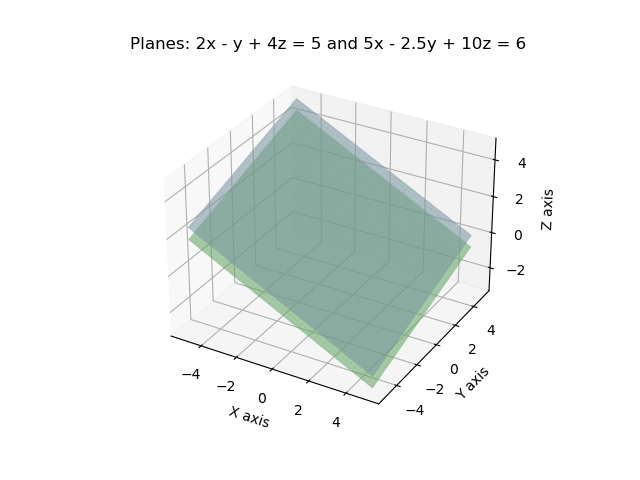
\includegraphics[width = 0.7\columnwidth]{figs/img.png}
    \caption*{}
    \label{figs}
\end{figure}

\end{document}